\documentclass[runningheads]{llncs}
\setcounter{tocdepth}{2}
\makeatletter
\renewcommand*\l@author[2]{}
\renewcommand*\l@title[2]{}
\makeatletter
%
\usepackage{listings}
\usepackage{float}
\usepackage{tikz}
\usepackage[T1]{fontenc}
\usepackage{graphicx}
\usepackage{hyperref}
\usepackage{color}
\renewcommand\UrlFont{\color{blue}\rmfamily}
\urlstyle{rm}
\def\UrlBreaks{\do\/\do-}
%
\begin{document}
%
\title{Kinode: A General-Purpose Sovereign Cloud Computer (DRAFT, PRIVATE)}
%
\titlerunning{Kinode – DRAFT, PRIVATE}
%
\author{
Benjamin McCormick \and
Nicholas B Ludwig \and
James Foley \and
Markus Vaas
}
\institute{Sybil Technologies AG}
%
\maketitle % typeset the header of the contribution
%
\begin{abstract}
Kinode is a software platform designed to integrate all facets of modern crypto application development.
Users can run their own services at both the interface and backend level.
Corporations or other entities can provide services in a permissionless, protocolized manner.
This node-based cloud computing model resolves the impedance mismatch between onchain protocols and web services.
Developers can write apps in any programming language that compiles to Wasm and easily distribute them to nodes.
The Kinode platform includes several components which will be described in this whitepaper: a virtual machine, an onchain global namespace, a utility token for governing and assigning value to that namespace, a PKI (Public-Key Infrastructure), a peer-to-peer networking protocol, a modular smart contract account system, and finally a governance apparatus to distribute onchain assets and continue development of the platform.
All of these components work in lockstep to solve the problems that have heretofore discouraged developers from embracing peer-to-peer computing.

\keywords{Operating System \and Decentralized \and Smart Contract Account \and Cloud \and Wasm \and Cryptocurrency \and Public-Key Infrastructure \and Namespace \and Peer-to-Peer }
\end{abstract}
%
\tableofcontents
%
%
%
%
\section{Overview}
\label{sec:overview}

Cryptocurrency, specifically smart contract blockchains, have triggered a nascent revolution in permissionless protocols: software in which all can participate and none can can shut down.
But progress towards a fully decentralized, permissionless internet has stagnated even as specific niches like decentralized finance flourish.
We believe that this progress is constrained less by blockchain speed and throughput than by an underdeveloped offchain computing substrate.

Recall the singular problem blockchains are designed to solve: preventing the double-spending of a cryptographically-owned asset.
\footnote{The Bitcoin whitepaper https://bitcoin.org/bitcoin.pdf describes using a distributed ledger to prevent double-spend of Bitcoin, and subsequent cryptocurrency projects generalized this to a blockchain preventing double-spend of arbitrary digital assets.}
The mechanism to achieve this, now well-proven, expanded to turing-complete VMs, and replicated dozens of times, is simple: signed transactions validated by a decentralized validator set and deposited into an append-only distributed ledger.

But what operations \textit{actually benefit} from an onchain transaction?

Permissionless finance obviously requires blockchains, at least at the moment of settlement.
Similarly for operations that mutate ownership of an asset.
Smart contracts have proven that double-spend prevention can productively be applied to any digital asset that requires guaranteed global consensus on the order and provenance of operations.

Which operations do not benefit from such guarantees?
For one, any action that only requires a signature from a single public key and does not need to be ordered:
a signed message from an individual, or an API published by an entity acting as the single source of truth.
Blockchain transactions are similarly unnecessary for actions undertaken between trusted parties, which, in fact, comprise a large portion of online communication.
It turns out that the category of networked operations that \textit{do not} require global consensus is much larger than the category of those that do benefit from being transactions.

Some protocols, like many in decentralized finance, function perfectly fine with no user interaction outside their onchain transaction protocol.
The user interface for such a protocol is merely a wrapper over the smart contract deployed onchain.
There is a vast landscape of possible protocols, however, which do not fit entirely into the purely-onchain paradigm.
Forcing these protocols into this model has led to countless failures.

Some believe that merely increasing transaction throughput by a few orders of magnitude (no small task) can resolve the issue by allowing transactions to be cheaply verified, even when they are not strictly necessary.
We do not.
There will always be significant relative costs to placing transactions in a globally-distributed ledger—not only monetary, but also in terms of latency, data storage, and compute overhead.
Transactions will \textit{always} present an impedence mismatch and be an inferior technical solution for operations that do not require global consensus.
Until we provide a proper platform for such operations, ``Web3'' will simply never outcompete ``Web2''.

\begin{figure}[H]
    \centering
    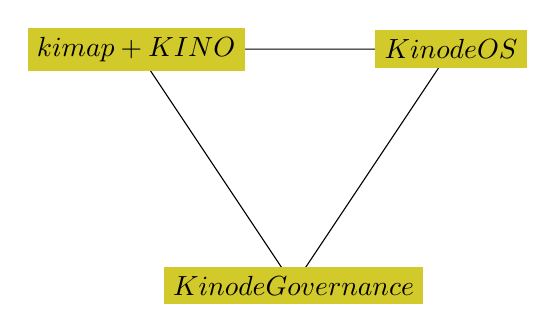
\begin{tikzpicture}
    \draw (0,3) node[fill=yellow!80!black]{$kimap+KINO$}
    -- (4,3) node[fill=yellow!80!black]{$Kinode OS$}
    -- (2,0) node[fill=yellow!80!black]{$Kinode Governance$}
    -- cycle;
    \end{tikzpicture}
    \caption{Architecture of Kinode.}
    \label{fig:triangle}
\end{figure}

The goal of the Kinode Hyperstructure
\footnote{https://jacob.energy/hyperstructures.html}
is to present a permissionless substrate for computing.
Smart contract blockchains provide access to global consensus state for provenance over digital assets–Kinode does ``everything else''.
In this paper, we present an operating system, an onchain global namespace, a value assignment and ranking mechanism, and the long-term governance structure for those components.

\section{Kimap}
\label{sec:kimap}

Historically, discoverability of both \textit{peers} and \textit{content} has been a major barrier for peer-to-peer developers.
Discoverability can present both social barriers (finding a new user on a game or chat) and technical obstacles (automatically acquiring networking information for a particular username).
Many solutions have been designed to address this problem, but so far, the ``devex'' (developer experience) of deploying centralized services has continued to outcompete the p2p discoverability options available.
Why is this?
\begin{enumerate}
    \item Libraries such as \verb|libp2p|, while effective at their goal of providing p2p primitives, do not provide the ``batteries included'' identity, discoverability, and network-effect-potential of more traditional centralized alternatives, and can also be difficult to approach for new developers.
    \item ``Pure'' peer-to-peer protocols still rely on hardcoded lists to bootstrap new entrants.
    \item Constructs such as distributed hash tables and CRDTs, frequently used in p2p protocols, are complex to properly implement.
    \item In order for a full, up-to-date snapshot of some globally-shared data to be easy to aquire, it should be stored in a single place.
    \subitem For Kinode, that ``one place'' is on a public blockchain inside a single smart contract.
    \subitem Multiple map contracts across multiple chains can be used to scale horizontally in the future while still providing a consistent interface to the global state.
    \subitem All data necessary to bootstrap peer-to-peer interaction must be available within this globally-shared map.
    \subitem Any ``missing piece'' required to complete handshakes or source peers will result in unreliability and re-centralization.
\end{enumerate}

Kimap is an onchain key-value store inspired by dmap
\footnote{https://github.com/dapphub/dmap}
, a minimalist onchain path-formatted key-value store.
It serves as the base-level shared global state that all nodes use to share critical signaling data with the entire network.
Like dmap, kimap is organized as a hierarchical path system and has mutable and immutable keys.
Several aspects of the minimal map implementation are customized for the ``namespace'' use case.

A brief description:

\begin{enumerate}
    \item All keys are strings containing exclusively characters 0-9, a-z (lowercase), - (hyphen).
    \item A key may be one of two types, a name-key or a data-key.
    \item Every name-key may create sub-entries directly beneath it.
    \item Every name-key is an ERC-721\footnote{https://eips.ethereum.org/EIPS/eip-721} NFT (non-fungible token),
    with a connected token bound account with a counterfactual address,
    that is a smart contract account implemented according to the ERC-7579\footnote{https://eips.ethereum.org/EIPS/eip-7579} standard.
    \item Every name-key may inscribe data in data-keys directly beneath it.
    \item All keys can be declared either mutable or immutable.
\end{enumerate}

For a complete specification, see Advanced Kimap in Section~\ref{sec:kimapadvanced}, which goes into detail regarding token bound accounts, sub-entry management, the use of data keys, and protocol extensibility.
For a description of the value-assignment mechanism that overlaps kimap, see Section~\ref{sec:kino} for the KINO utility token.

\subsection{Example Kimap Entries}

\begin{figure}[H]
    \centering
    \begin{verbatim}
    os
        foo
            ~ip
            ~ws-port
            ~net-key
        bar
            ~routers
            ~net-key
    kino
        baz
            package
                ~metadata-hash
                ~metadata-uri
    eth
        alice
            ~routers
            ~net-key
        bob
            ~routers
            ~net-key
    \end{verbatim}
    \caption{Example kimap.}
    \label{fig:example kimap}
\end{figure}

Fig.~\ref{fig:example kimap} shows an example with three top-level ``zones'', \verb|eth|, \verb|kino|, and \verb|os|.
Below those are a number of namespace entries: \verb|foo|, \verb|bar|, and \verb|baz|.
The full path for \verb|foo|'s \verb|~ip| sub-entry would be \verb|~ip.foo.os|.

In this paper, we will sometimes use the term ``domain'' interchangeably with what we refer to here as a ``namespace entry''.
This is a useful shorthand, and in many ways, kimap does mirror the role of DNS in the worldwide web.
However, the domain analogy is inaccurate if applied directly to all namespace entries because not all namespace entries resolve to a networking protocol target.

E.g., only entries containing \verb|~net-key| are used by the KNS (Kinode Name System) which runs \textit{on top} of kimap.
Entries \verb|baz.kino| and \verb|package.baz.kino| have no data keys to describe their status in the KNS, and so the ``domain'' analogy breaks down for them.
The design of kimap is generic in the sense that many protocols are expected to share this global namespace for different purposes.
The specification of KNS itself, as a protocol operating on kimap, is described in Section~\ref{sec:kns}, as is the specification of the Kinode Package Manager, Section~\ref{sec:packagemanager}, both of which make an appearance in this example.

\section{KNS: Kinode Name System}
\label{sec:kns}

Kinode Name System is a protocol built on top of kimap that acts as a PKI for the network.
KNS transforms an entry in the kimap namespace into a \textit{node identity} for use in the Kinode network, where a node is an instance of Kinode OS, able to communicate peer-to-peer with other such nodes.
Node identities are central to the programming model of Kinode OS.
Usually manipulated as strings in a process, a node identity is the first component of an \verb|address|, which uniquely identifies a specific process running on that node, part of a package, published by some node. See Section~\ref{sec:os} for definitions and discussion.

\subsection{Specification}
\label{sec:knsspec}

The definition of a node identity in the KNS protocol is any kimap entry that has:

\begin{enumerate}
    \item A \verb|~net-key| sub-entry AND
    \item \begin{enumerate}
        \item A \verb|~routers| sub-entry OR
        \item An \verb|~ip| sub-entry AND at least one of:
            \begin{enumerate}
                \item \verb|~tcp-port| sub-entry
                \item \verb|~udp-port| sub-entry
                \item \verb|~ws-port| sub-entry
                \item \verb|~wt-port| sub-entry
            \end{enumerate}
        \end{enumerate}
\end{enumerate}

A sample of this protocol can be seen in Fig.~\ref{fig:example kimap}.
Two classes of nodes are defined: \textit{direct} and \textit{indirect}.
Direct nodes are those that publish an \verb|~ip| and one or more of the \verb|port| sub-entries.
Indirect nodes are those that publish \verb|~routers|.
The nature of direct and indirect nodes in networking is described in Section~\ref{sec:osnetworking}.

The data stored at \verb|~net-key| must be 32 bytes corresponding to an Ed25519 public key.
This is a node's signing key which is used across a variety of domains to verify ownership, including in the end-to-end encrypted networking protocol between nodes.
The owner of a namespace entry/node identity may rotate this key at any time by posting a transaction to kimap mutating the data stored at \verb|~net-key|.

The bytes at a \verb|~routers| entry must parse to an array of UTF-8 strings.
These strings should be node identities.
Each node in the array is treated by other participants in the networking protocol as a router for the parent entry.
Routers should themselves be direct nodes.
If a string in the array is not a valid node identity, or it is a valid node identity but not a direct one, that router will not be used by the networking protocol.
Further discussion of the networking protocol specification is presented in the Section~\ref{sec:osnetworking}.

The bytes at an \verb|~ip| entry must be 16 big-endian bytes corresponding to a 128-bit unsigned integer.
This integer is interpreted as an IPv4 address if it is <32-bit.
Otherwise it is interpreted as an IPv6 address.

Lastly, the bytes at any of the following port entries must be 2 big-endian bytes corresponding to a 16-bit unsigned integer:

\begin{enumerate}
	\item \verb|~tcp-port| sub-entry
	\item \verb|~udp-port| sub-entry
	\item \verb|~ws-port| sub-entry
	\item \verb|~wt-port| sub-entry
\end{enumerate}

These integers are translated to port numbers.
In practice, port numbers used are between 9000 and 65535.
Ports between 8000-8999 are usually saved for HTTP server use.

\subsection{Indexing}
\label{sec:knsindexing}

Events emitted by kimap are used to index map data.
Kinode OS provides all the primitives required to index effectively in a userspace application, and the default distribution of the OS includes a process which indexes kimap for the purpose of reporting KNS data to the networking protocol module.

\subsection{Adding Other Onchain Identity Primitives}
\label{sec:knsotherprimitives}

The KNS is not an attempt at replacing or competing with existing onchain identity primitives such as ENS and Lens.
Rather, it is designed to satisfy the public key infrastructure needs of the Kinode network.
It is of paramount importance that nodes can initiate secure communication with one another without the use of any data other than what is available publicly onchain.
Peer-discovery middlemen induce centralization and complicate networking protocols.

The structure of kimap means that KNS avoids competition with other identity primitives by seamlessly integrating them.
As of this paper, this has already been done for ENS protocol.
Here is a brief description of the procedure to do so:
\begin{enumerate}
    \item Create a contract to allow owners, and only owners, of a given identity primitive to mint their corresponding name in a kimap namespace controlled by this contract.
    \item Mint and transfer the top-level namespace entry corresponding to an outside identity primitive, \verb|lens| for example.
    \item If necessary, configure LayerZero, or other such cross-chain messaging protocol, to allow owners of an identity primitive on another chain to verify their ownership on the chain that kimap is deployed on.
    \item The final result is that the owner of, for example, \verb|myname.lens| can exclusively register \verb|myname.lens| in kimap, add a \verb|~net-key| sub-entry, and use it as their PKI entry for Kinode.
\end{enumerate}

\section{Kinode OS}
\label{sec:os}

This section discusses the architecture of Kinode OS.
For a more ``hands-on'' description of the OS, including detailed programming examples and documentation, go to \href{https://book.kinode.org/}{book.kinode.org}.

Kinode OS is a process virtual machine run to operate a ``node'' on the Kinode network.
At its core, the virtual machine wraps around a Wasm runtime
\footnote{Wasm is specified at https://webassembly.github.io/spec. Kinode uses Wasm for processes because it is a highly performant, language independent, portable, and sandboxable compilation target.}
which executes all userspace code.
After a node identity is registered onchain in the KNS, the operator should boot the OS using the private key matching the public \verb|~net-key| posted in the kimap during registration.
Once this has been done, if the networking details (routers, IP, etc) are properly read from the kimap and matched by the runtime, that node is now ``online''.
Other nodes can interact with the booted node through the Kinode networking protocol by reading its KNS node identity and using the data stored there.

The runtime is as simple as possible, with a maximal amount of logic ejected to userspace.
In the future, Kinode will benefit from ``client diversity'' as does a traditional blockchain: many implementations of the virtual machine
\footnote{The Wasm runtime is by a wide margin the most complex aspect of the OS, and at least a dozen such runtimes exist today, written in multiple languages.
This bodes well for future Kinode client diversity.}
will make the network more resilient to potential bugs and decentralize the development process, leading to productive ossification of core features, stability, and long-term strength.

While all packaged into a single executable, the OS can productively be described in 3 parts: a \textit{runtime}, a set of \textit{runtime modules}, and \textit{userspace}.
The ``kernel'' frequently referred to in this paper is in fact just a runtime module.

The runtime is a ``native'' (to whatever architecture it targets, which may be Unix, a browser, hardware...) program that manages node booting (including onchain registration) and (generally asynchronously or in parallel) executes the runtime modules.
Runtime modules are blocks of code written at the same level of abstraction as the runtime itself, but designed to resemble userspace processes.
These modules are registered in the kernel \textit{as} processes, meaning that they can be messaged by userspace in the system-wide request-response protocol and secured via capabilities.
Finally, userspace is comprised of all non-runtime-module processes executed virtually by the kernel.
Userspace processes are always compiled to Wasm and comport to the Wasm Component Model\footnote{https://component-model.bytecodealliance.org/}.
They are adapted to the Kinode WIT file which defines the common interface that all processes must implement and provides a set of ``system calls'' afforded to userspace processes by the kernel.

The reference implementation is currently written in Rust, as are all the runtime modules.
It also comes with a number of pre-installed userspace packages that perform critical tasks.
In the future, other entities will likely seek to distribute their own implementations which may contain different pre-installed packages or even different runtime modules.

\begin{figure}
    \centering
    \begin{lstlisting}
    eth:distro:sys
    http_client:distro:sys
    http_server:distro:sys
    kernel:distro:sys
    kv:distro:sys
    net:distro:sys
    state:distro:sys
    terminal:distro:sys
    timer:distro:sys
    sqlite:distro:sys
    vfs:distro:sys
    \end{lstlisting}
    \caption{The full list of runtime modules in the OS distribution maintained by core developers as of this writing.}
    \label{fig:runtime modules list}
\end{figure}

\subsection{WIT}
\label{sec:oswit}

Wasm Interface Type\footnote{https://component-model.bytecodealliance.org/design/wit.html}, or WIT, is a language to describe types and function definitions which can be used in a Wasm component.
Kinode OS uses a single WIT file to define the types shared across all processes and provide a number of functions.
The functions fall into three categories:
\begin{enumerate}
    \item Self-configuration
    \item Capabilities management
    \item Message I/O
\end{enumerate}

WIT files are organized into ``worlds''. All types and functions provided to Kinode processes are currently stored in one world labeled \verb|lib|.
In a separate world, \verb|process|, a single function named \verb|init| is exported, which means that all Wasm apps that use the \verb|process| world must implement that function.
It is the entry point by which the Kinode kernel starts executing a process.

\subsubsection{WIT Types}
\label{sec:oswittypes}

Discussion of the types presented here will occur throughout the rest of the OS description.
Some types in kinode.wit are omitted for brevity or because they are discussed later.

\begin{figure}[H]
    \centering
    \begin{verbatim}
    // JSON is passed over Wasm boundary as a string.
    type json = string;

    type node-id = string;

    type context = list<u8>;

    record process-id {
        process-name: string,
        package-name: string,
        publisher-node: node-id,
    }
    record address {
        node: node-id,
        process: process-id,
    }
    record lazy-load-blob {
        mime: option<string>,
        bytes: list<u8>,
    }
    \end{verbatim}
    \caption{Basic types in kinode.wit}
    \label{fig:WIT Types 1}
\end{figure}

An \verb|address| globally identifies a process running on a particular node.

A \verb|process-id| identifies a particular process by its publisher, package name, and process name.

\subsubsection{WIT Host Functions}
\label{sec:oswitfuncs}

WIT host functions must be implemented by the kernel.
The Wasm Component model allows these functions to be called by processes.

\begin{figure}[H]
    \centering
    \begin{verbatim}
    // self-configuration
    print-to-terminal()
    set-on-exit()
    get-on-exit()
    get-state()
    set-state()
    clear-state()
    spawn()

    // capabilities management
    save-capabilities()
    drop-capabilities()
    our-capabilities()

    // message I/O
    receive()
    get-blob()
    send-request()
    send-requests()
    send-response()
    send-and-await-response()
    \end{verbatim}
    \caption{Host functions in kinode.wit}
    \label{fig:WIT Functions}
\end{figure}

\subsubsection{WIT Process Format}
\label{sec:oswitprocess}

The process format enforced by kinode.wit is remarkably simple: it imports the types and functions defined in the main library world, and requires processes to implement a single function: \verb|init|.
\footnote{This does not preclude processes from implementing other functions.}

\begin{figure}[H]
    \centering
    \begin{verbatim}
    world process {
        include lib;
        export init: func(our: string);
    }
    \end{verbatim}
    \caption{Process world in kinode.wit}
    \label{fig:Process world}
\end{figure}

\verb|init| serves as the entry point for a process.
The kernel begins execution of a process by calling \verb|init|.
When \verb|init| returns, the process will cease execution.
\footnote{All processes are single-threaded. To perform parallel computation, one can spawn child processes.}

\subsection{Microkernel}
\label{sec:osmicrokernel}

Every aspect of the operating system, including the kernel itself, comports to a set of messaging rules defined by the microkernel\footnote{A microkernel architecture is ideal for a ``Wasm OS'' because it allows a maximal amount of system logic to live in Wasm itself, allowing system code to experience all the safety and conveniences afforded to userspace processes. See \href{https://wiki.osdev.org/Microkernel}{https://wiki.osdev.org/Microkernel}} which is responsible for five things:
\begin{enumerate}
    \item Using a Wasm runtime
    \footnote{The reference implementation currently uses \href{https://wasmtime.dev}{Wasmtime}.}
    to execute compiled processes which implement the Kinode WIT standard, where execution includes managing their memory usage.
    \item Implementing the host functions, exposed to all processes, defined in Kinode WIT standard.
    \item Implementing the kernel API that allows processes with kernel-messaging capabilities to perform aspects of process management.
    \item Passing messages between all processes including to/from the kernel itself.
    \item Enforcing messaging capabilities.
\end{enumerate}

Messaging capabilities are a subset of the capabilities security model defined by the OS, issued by the kernel process, \verb|kernel:distro:sys|.
Each process can mark itself as either \verb|public| or \verb|private| at instantiation.
Public processes can be messaged by any other process.
Private processes, as enforced by the kernel, require that the message source holds their messaging capability.
See the discussion of capabilities in Section~\ref{sec:oscapabilities} for details on their use and how capabilities apply to processes running a remote node.

As of this writing, the kernel runtime module in our reference implementation of the OS fits into about 2,700 lines of Rust.

The kernel is responsible for maintaining backwards compatibility.
If a process was written for an older version of the kernel (which is determined by the version number of the WIT file it implements), newer kernels must store that WIT version and match it to the process.
If data structures in the WIT file change between versions, the kernel is responsible for translating between formats.
This kind of upgrade is possible but unlikely once the kernel reaches version 1.0.

\subsection{Message Passing}
\label{sec:osmessagepassing}

A message between two Kinode processes is either a request or a response.
A message has a single source \verb|address| and a single target \verb|address|.

\begin{figure}[H]
    \centering
    \begin{verbatim}
    record request {
        inherit: bool,
        expects-response: option<u64>,
        body: list<u8>,
        metadata: option<json>,
        capabilities: list<capability>,
    }
    record response {
        inherit: bool,
        body: list<u8>,
        metadata: option<json>,
        capabilities: list<capability>,
    }
    variant message {
        request(request),
        response(tuple<response, option<context>>),
    }
    \end{verbatim}
    \caption{Message type in kinode.wit}
    \label{fig:WIT Types 2}
\end{figure}

Messages are produced and consumed by Kinode processes.

If the node identity indicated in the target \verb|address| matches that of the local kernel or is simply the string \verb|our|, the message is routed directly through the kernel to the target (assuming the source has the capability to message the target or the target is public).
Otherwise, the message is routed through the networking runtime module, \verb|net:distro:sys|, to the remote node indicated.

Ordering of messages between a given source and a given target is enforced by both kernel and networking protocol.
Messages are not otherwise ordered, meaning that if process A sends messages 1, 2, 3 to process B, and process B sends messages 4, 5, 6 to A, no guarantees are enforced other than that process B will receive messages 1, 2, 3 in that order and process A will receive 4, 5, 6 in that order.
If process C sends message 7 to A, it may be received before 1, after 3, or somewhere in between.

Message delivery is not guaranteed.
If a message targets a local process, the target may crash or the kernel may suspend execution between message creation and delivery.
Far more treacherous is delivery of messages to remote processes.
Nodes may go offline, experience network congestion, or otherwise drop incoming messages.
\footnote{Computer networking, being a fundamentally physical process, is impossible to effectively abstract over without failure modes, because the physical world imposes them.}
To this end, two error modes are baked into Kinode message passing: offline and timeout.

Requests can be sent at any time, while responses must target a process that has a matching outstanding request.
A request is outstanding if:
\begin{enumerate}
    \item it expects a response
    \item its timeout has not expired
\end{enumerate}
Every request that expects a response must set a timeout value, measured in seconds.
The kernel is responsible for returning a timeout error to a request which expects a response and does not get matched to one within the number of seconds declared.
\footnote{Timeouts must be viewed as a lower bound, as in, the kernel will not return a timeout error for at least X seconds. The upper bound cannot be guaranteed.}

The offline error type is only returned by \verb|net:distro:sys|.
It may be returned if the node that a request targets is definitively unreachable.
This may occur if a direct node's networking information in KNS is invalid, an indirect node has no routers, a node refuses all networking protocol connections / does not comport to protocol, or any other such immediate error.
In practice, ``offline'' and ``timeout'' can usually be treated the same way: by a combination of alerting the program user and retrying the message.

Protocols for retrying a message, particularly to a remote process, are left to userspace.
Different applications are best served by different retry strategies:
a one-off message may be awaited in a blocking fashion, surfacing an error to the sender's UI.
A message that's part of a large data transfer may not expect a response at all, instead relying on the final message in the transfer to await a response.
The networking protocol's role as a general-purpose messaging system means that it must support all of these use cases and more.

\subsection{Capabilities-Based Security}
\label{sec:oscapabilities}

Kinode OS uses capabilities\footnote{Capabilities are ``unforgeable tokens of authority'', validated by the kernel, that allow processes to acquire privileges both at the runtime and userspace level.
See the paper ``Capability Myths Demolished'' for a good introduction to the topic.}
to enable sensible security between both userspace processes and runtime modules.
Security between programs is directly related to the sovereignty goals of the OS: a user must be able to install a program without needing to evaluate its source code or blindly trust its developer.
Wasm programs are sandboxed, but have access to powerful tools including networking, memory, CPU, and disk space, not to mention the possible secrets they contain (consider a wallet program).
Not only must these tools be granted to programs on a case-by-case basis, but without some form of control between sandboxed programs, the sandbox becomes pointless, as any power or secret knowledge granted to a given program could be accessed by other programs!

\begin{figure}[H]
    \centering
    \begin{verbatim}
    record capability {
        issuer: address,
        params: json,
    }
    \end{verbatim}
    \caption{Capability type in kinode.wit}
    \label{fig:WIT Types 3}
\end{figure}

Capabilities are signed by the local kernel's \verb|~net-key| to convert them into unforgeable tokens of authority.
Processes don't need to concern themselves with verifying signatures.
Instead, the kernel filters out local capabilities which are not properly signed.
If a process is in possession of a capability, it may send it to another process.
Remote capabilities–capabilities created by a different kernel–are not verified.
Why not?
If an invalid remote capability is created and passed in a message, the holder will be alerted to its invalid nature if/when the holder tries to use it.

As elaborated on in Section~\ref{sec:packagemanager}, which describes a package manager for Kinode, software written on Kinode OS will often benefit from declaring a set of capabilities desired at the time of install.
Many of the built-in runtime modules distributed with the OS, including the kernel itself, have a capabilities protocol.
The kernel's capabilities protocol is part of the OS specification because it applies to every process and is the bedrock security model of the OS.
It is also very simple:
\begin{enumerate}
    \item Upon instantiation, every process is given its own \textit{messaging capability}.
    \item Every process may mark itself as \verb|public|.
    \item A messaging capability is defined as a capability with the \verb|issuer| field set to the process in question, and the \verb|params| field set to the string \verb|"messaging"|\footnote{Quotation marks included here to produce valid JSON, as is best practice for the params field.}
    \item If a process is public, the kernel will pass any message to it. If not, the kernel will check that local processes sending requests to this process are in possession of the messaging capability.
\end{enumerate}

Note that remote processes are not filtered by messaging capabilities.
Because other kernels can spoof such information as process names, it does not make sense to filter by process name for a remote message.
Instead of using messaging capabilities to filter remote processes, a process instead may decide whether or not it accepts messages from remote sources in general, and then filter by the identity of the source node which cannot be spoofed.

\subsection{System Primitives}
\label{sec:osprimitives}

Kinode OS manages four primitives via runtime modules:

\begin{enumerate}
    \item Networking: sending encrypted messages between nodes using permanent cryptographic identities.
    \item Data Persistence: writing to disk with the option to use remote backup systems.
    \item Global Consensus State: integrating with blockchains to read data and write transactions.
    \item Web: HTTP client and server.
\end{enumerate}

The commonality between these four items is the requirement for I/O.
Therefore, they cannot be built as userspace Wasm processes.
Instead they are written as runtime modules: chunks of code at the same native level of the runtime and specially registered as processes in the kernel, which itself is a runtime module.

Networking, data persistence, blockchain access, and HTTP read/write are all presented to userspace processes as a request-response API between a runtime module and the process using the primitive.
See Fig.~\ref{fig:runtime modules list} for a full list of the process IDs which present these primitives.
The API for a given runtime module included in the \verb|distro| package is part of the set of interfaces grouped within the Kinode OS versioning system.
The OS uses a single semantic versioning number to indicate breaking and non-breaking changes to these APIs, the kernel, the KNS/kimap onchain protocols, and the networking protocol.
This is covered further in the discussion of backwards compatibility in Section~\ref{sec:osbackwardscompat}.

A few not-strictly-necessary but useful I/O primitives are also presented as APIs via runtime modules.
These are: a terminal, a timer, and the advanced data persistence options of SQlite, a key-value store, and a virtual filesystem.

Kinode OS can expose new primitives at the runtime level via \textit{extensions}, covered in Section~\ref{sec:osextensions}.

\subsection{Example Process}
\label{sec:osexampleprocess}

Now that the OS has been described in the abstract, and before we dive in to the specific designs of various runtime modules, it may be helpful to provide a code sample showing what a process actually looks like.

\begin{figure}[H]
\begin{verbatim}
wit_bindgen::generate!({
    path: "wit",
    world: "process-v0",
});

struct Component;
export!(Component);

use crate::kinode::process::standard::print_to_terminal;

impl Guest for Component {
    fn init(our: String) {
        print_to_terminal(0, "hello from a process");
        print_to_terminal(
            0,
            &format!("our process-id: {our}")
        );
    }
}
\end{verbatim}
    \caption{A process implemented in Rust}
    \label{fig:example process}
\end{figure}

By generating bindings from \verb|kinode.wit|, a process acquires a set of types and functions from the langauge in which it is written.
The types and functions generated are often cumbersome to use directly due to their basic nature–in practice nearly all processes will use a library written for their particular langauge that smooths over the WIT interface and provides helper functions, type implementations, and so on.
\footnote{ As of this writing, most processes have been written in Rust and an extensive library of this description has already been written, available at https://github.com/kinode-dao/process\_lib }
To generate WIT bindings, it is merely required to import \verb|kinode.wit| and use the guest language's tooling, in the case of this example wit-bindgen\footnote{https://github.com/bytecodealliance/wit-bindgen} for Rust.

\subsection{Selected Runtime Modules}
\label{sec:osmodules}

This section describes a number of runtime modules of critical importance.

\subsubsection{Virtual Filesystem}
\label{sec:osvfs}

The OS ships with \verb|vfs:distro:sys|, a module which presents a standard filesystem API accessible to all processes with the capability to message it.
Directories and files created in the VFS are saved on the host machine's filesystem.
All I/O is mediated by the VFS, allowing processes to abstract away management of filesystem resources.

All processes that wish to persist data locally between boots will use either the VFS or another runtime module that writes to disk, which may be an extension or one of the default-distribution's SQLite or key-value store modules.

\subsubsection{Networking}
\label{sec:osnetworking}

This runtime module is the part of the OS which implements the Kinode networking protocol.
This module is somewhat special: in the kernel, messages with a \verb|target| that contains a node identity other than that of the kernel are all routed to \verb|net:distro:sys|.
Once a message is passed to the networking module, it is routed to the target node using the information available in the Kinode Name System.
For this reason, the networking module \textit{must} be made aware of the current onchain state of the KNS.

KNS updates are given to \verb|net:distro:sys| using a request API made available to processes that have messaging capabilities to it.
Note that messaging capability to \verb|net| is only required to send configurational messages, and is not required to simply send networked messages: those are handled through the kernel.
Note also that as the KNS state grows, it will become prudent to not load the entire state into the networking module, but rather dynamically query the state as networking information is required for accessing new nodes or updating stale data from known ones.

The networking protocol itself will not be fully specified here, as it is still being finalized and is best suited by its own document. However, some key aspects:

\begin{itemize}
    \item The protocol uses exclusively information available onchain, including IP addresses, ports, and router nodes, to faciliate message-passing.
    See the description of KNS in Section~\ref{sec:kns}.
    \item Direct nodes publish their routing information onchain.
    Indirect nodes publish a set of routers who faciliate message-passing for them.
    This is analogous to STUN+TURN in WebRTC.
    A router may be able to facilitate a direct connection for indirect nodes in a STUN-like manner.
    \item Networking may occur across many underlying transport protocols.
    The specification of KNS in the kimap allows for a node identity to publicize the port to be used for each transport protocol that node supports.
    The runtime is responsible for implementing each protocol that a node broadcasts.
    In practice, nodes will mostly use TCP for direct communication and routers will support a variety of protocols used by special-purpose nodes (such as mobile devices or nodes running in-browser).
    \item Messages are end-to-end encrypted using a Noise protocol
    \footnote{http://www.noiseprotocol.org/noise.html}
    where each node has a static public key in their Ed25519 key published onchain, the cipher function is ChaChaPoly, and hash function is BLAKE2s.
    The XX pattern is used for handshakes.
    \footnote{This is described in Noise as ``Noise\_XX\_25519\_ChaChaPoly\_BLAKE2s''.}
    \item Message-passing in a networked context aims to be as similar as possible to the local context.
    However, the offline and timeout error-cases together cover the inescapable realities of networking.
    \item There are no ACKs at the Kinode protocol level: if the underlying transport protocol confirms delivery, failure to do so can become an offline error.
    Otherwise, the request-response pattern must be used to confirm message delivery.
\end{itemize}

\subsubsection{HTTP Client \& Server}
\label{sec:oshttp}

Web access is a critical part of many programs that run on Kinode.
A built-in HTTP client module allows processes to ingest data from the web.
The HTTP server module allows processes to serve data to the web, either statically by sending a payload to be served for a given path, or dynamically by requesting the server module to forward incoming HTTP requests to the process.
Both modules present a request-response API (documented elsewhere).

Most programs that present an interface to the node user do so through a combination of static and dynamic HTTP server path bindings.
All paths bound by a process are prefixed with the \verb|process-id|, in order to remove the possibility of collisions or imposter resources.
Further, paths may be bound as ``authenticated'', meaning that access will require a JSON Web Token (JWT) given via password login to the node.
Once the token is acquired via login, a user may access any authenticated path served by processes on the node.

This raises a subtle security issue: if a process serves an API allowing the user to perform various actions over HTTP (as is quite common), other processes running on the same node can easily access the API by serving a frontend JavaScript file of their own, which can fetch content from any authenticated path on the node.
This circumvents the capability-based security model applied to inter-process communication and suddenly shifts the trust assumptions for all software installed on a node that acquires the capability to message the HTTP modules.

Rather than allow this escalation of trust assumptions, the HTTP server provides a special mechanism to serve authenticated paths that are only accessible at a \textit{subdomain}.
The security model of the browser is thus leveraged to generate a new JWT for the subdomain URL, required for access to the paths at the subdomain and disallowing client access from the base domain.
Users may then login at the subdomain with the same password as the base node server and generate a new token in their browser.
We call this model ``Secure Subdomains''.
Processes that serve sensitive HTTP APIs for user interfaces are encouraged to use Secure Subdomains to properly sandbox these operations away from other software running on the user's node.

\subsubsection{ETH RPC}
\label{sec:oseth}
The OS includes an Ethereum (and EVM-compatible chains) indexing runtime module, \verb|eth:distro:sys|, which provides read and write access to blockchain data. This module can connect directly to WebSocket RPC endpoints or relay through other Kinode nodes, forming a potential chain of relays.

The module implements standard Ethereum JSON-RPC API methods, supporting operations such as querying block data, retrieving account balances, estimating gas costs, and sending transactions. Processes interact with this module through a request-response API, typically using a \verb|Provider| struct that encapsulates chain-specific details and request handling.

Optional \verb|.eth_providers| and \verb|.eth_access_settings| JSON files in the node's home folder may be used to configure the module. The former allows users to specify their preferred RPC endpoints, relay nodes, and chain-specific settings, and the latter controls whether other nodes may use this node as a provider with potential allow/deny lists. The configuration can also be modified at runtime through the module's API, enabling flexible provider management.

The module supports both one-time requests and subscriptions, particularly useful for monitoring real-time events specific log entries or kimap note keys. Subscriptions are managed through unique identifiers, allowing processes to filter and unsubscribe from event streams as needed.

\verb|eth:distro:sys| also integrates with Kinode-specific functionalities, such as querying the kimap contract, which is central to Kinode's naming and identity system. This allows processes to interact with Kinode-specific on-chain data seamlessly.

\begin{verbatim}
let node = namehash("node.foo.os");
let (tba, owner, note) = provider.kimap_get(&node)?;
\end{verbatim}

The module acts as a relay and subscription manager for Ethereum JSON-RPC requests and responses. Processes may use helper functions and structs to format requests according to the Ethereum JSON-RPC specification\footnote{\url{https://ethereum.github.io/execution-apis/api-documentation/}}.

\verb|eth:distro:sys| handles maintenance of subscriptions, managing provider connections, and facilitating the routing of Ethereum data between Kinode instances, allowing processes to have direct control over their Ethereum interactions while benefiting from the module's network management capabilities, including the ability to relay requests through other nodes when direct RPC access is unavailable or not yet configured.

This design facilitates the development of decentralized applications that can efficiently interact with global blockchain networks, even in constrained peer-to-peer environments. It allows for unique scaling possibilities:

\begin{itemize}
	\item Applications can default to public endpoints while allowing users to easily switch to their own nodes.
	\item Nodes without direct RPC access can relay through peers, distributing network load.
	\item Multi-chain applications can be built with a unified interface, simplifying development across different EVM-compatible networks.
\end{itemize}

By providing this flexible and powerful interface to Ethereum and other EVM chains, Kinode OS enables developers to create robust blockchain-integrated applications while giving users control over their blockchain access points.

\subsubsection{SQLite, KV-Store}
\label{sec:osdbs}

In addition to the VFS, the OS provides SQLite and key-value store runtime modules.
These modules serve as high-performance disk storage options for processes that require persistence.
Each module has a request-response API (documented elsewhere) exposing their respective operations.
Both SQLite and KV-store structure requests such that processes with the default messaging capability may create and access only their own tables.
Of course, processes may use other storage options designed in userspace or as runtime extensions.

\subsection{Runtime Extensions}
\label{sec:osextensions}

Wasm is an excellent compilation target for processes.
Processes are naturally sandboxed and cross-platform.
However, there are also costs associated with Wasm.
For example, not all libraries can be compiled to Wasm and hardware support for accelerators like GPUs is currently lacking.
Extensions supplement and compliment Kinode processes, removing these constraints, while maintaining the advantages associated with kernel-provided services, e.g., the request/response system.

Extensions are simply WebSocket clients, written in any language and run natively alongside Kinode OS, that connect to a paired process.
The paired process serves as the interface between the extension and the rest of the Kinode system.

Extensions can be written in any language and can use any library, since an extension is just a native program that can connect to Kinode as a WebSocket client and that implements a certain protocol.

The cost of extensions is that they are not as easy for users to install and use.
Since they are native, rather than Wasm, they will not run on arbitrary systems.
They are also not as easy to distribute as packages.
Therefore only sophisticated users should be expected to run extensions, since they will either need to compile them themselves or set up and maintain an additional program running next to Kinode.

\subsection{Backwards Compatibility}
\label{sec:osbackwardscompat}

Once the OS reaches version 1.0, no backwards-incompatible change will be allowed in a subsequent version.
The surface area presented by the OS for the purpose of backwards-compatibility is defined as:
\begin{itemize}
    \item The networking protocol
    \item The request-response API for each runtime module listed in Figure~\ref{fig:runtime modules list}
    \item kinode.wit and the kernel-level implementation of the host functions
    \item The on-disk footprint of runtime modules that use disk, along with the encrypted keyfile used by the OS to store the networking key and JSON Web Token used for authenticating of node-served frontends.
\end{itemize}

A number of userspace packages included in the reference distribution must also be backwards-compatible due to the inconvenience created by breaking changes.
This includes \verb|app_store:sys|, \verb|homepage:sys|, and \verb|terminal:sys|.

\section{Package Manager}
\label{sec:packagemanager}

Like KNS, the Kinode Package Manager is a protocol deployed on kimap.
It is another protocol critical to the operation of Kinode OS.
As described in Section~\ref{sec:os}, the userspace presented by the OS is comprised of processes, which are bundled into packages.
There is no kernel-level method for managing the packages installed in a node.
Rather, userspace programs with the required capabilities must save packages in the virtual filesystem and prompt the kernel to start running certain processes.

If a process has the necessary capabilities, they may create requests to and receive responses from \verb|kernel:distro:sys| like any other process.
The kernel specifies a request type that includes commands relevant to managing processes.
Programs that wish to ``install'' and ``uninstall'' processes merely submit these requests.
These programs must also have capabilities to access the virtual filesystem, such that they can create new top-level directories formatted in such a way that the kernel can access compiled \verb|.wasm| files that contain a single process.

By convention, packages are stored in a \verb|.zip| file with the full name of the package \verb|<package_name>:<publisher_node_id>|, e.g., for a chat app \verb|chat| published by \verb|template.os|, the full name of the package is \verb|chat:template.os|.
The top level of the zipped directory contains a \verb|pkg| directory and optionally a directory for the source code of each process defined in the \verb|pkg| directory.
The \verb|pkg| directory defines processes by
\begin{enumerate}
    \item Containing a \verb|.wasm| file, the name of which matches the process name
    \item Optionally declaring the process in a file named \verb|manifest.json|, which defines the processes in the package that should be run upon installation and when a node with this package installed is first booted.
\end{enumerate}

\verb|pkg| may also contain a \verb|scripts.json| file which defines a list of processes that can be run as scripts.
Scripts are merely processes that, by convention, can be executed from the system terminal, run for some period of time, and, before exiting, optionally return a final response, which the terminal may print.

It is important to note that all of the above logic exists outside of the kernel and runtime.
A package's directory, metadata, and manifest are all interpreted by userspace code and boiled down to a series of kernel commands including \verb|InitializeProcess|, \verb|RunProcess|, and \verb|KillProcess|.
Of course, Kinode OS would not be very useful without this logic, and so the distribution maintained by core developers comes with a combination app store and package manager called \verb|app_store:sys|.
Note that the publisher name, \verb|sys|, is not a node identity.
The publisher value in a package name is not enforced by the kernel.
It is accepted uncritically, and it is again the responsibility of the userspace package manager to assert a valid publisher if desired.

\subsection{Specification}
\label{sec:packagemanagerspec}

The userspace app store/package manager maintained by core developers uses an onchain protocol running on kimap to enable app discoverability and ranking.
The definition of a package (interchangeably called an ``app'') in this protocol is any kimap entry which has both of the following sub-entries:

\verb|~metadata-hash|, \verb|~metadata-uri|.

The publisher name of a package is the parent-parent entry.
The package name is the last path item in the parent entry.

A \verb|~metadata-hash| entry must contain 32 big-endian bytes corresponding to a SHA-256 hash of the \verb|metadata.json| file used to install a package.

A \verb|metadata-uri| entry must contain a UTF-8 string: a Uniform Resource Identifier (URI) indicating where the metadata file can be found (which, when hashed, matches \verb|~metadata-hash|).

\begin{figure}[H]
    \centering
    \begin{verbatim}
    os
        foo
            ~ip
            ~ws-port
            ~net-key
            foos-app
                ~metadata-hash
                ~metadata-uri
    kino
        bar
            baz
                ~metadata-hash
                ~metadata-uri
            bam
                ~net-key
                ~routers
                ~metadata-hash
                ~metadata-uri
                boozle
                    ~metadata-hash
                    ~metadata-uri
    \end{verbatim}
    \caption{Example kimap with multiple packages present.}
    \label{fig:example kimap with packages}
\end{figure}

In Fig.~\ref{fig:example kimap with packages} there are 4 packages present: \verb|foos-app:foo.os|, \verb|baz:bar.kino|, \verb|bam:bar.kino|, and \verb|boozle:bam.bar.kino|.
Note that the parent path from a valid package sub-entry contains the entire package name including publisher.
Note also that a publisher does not need to be a valid node identity as defined in the KNS protocol, though in practice it likely will be.
A single publisher providing multiple packages can do so by minting sub-entries corresponding to those packages' names.
Lastly, a package may also itself be a node identity as demonstrated in \verb|bam.bar.kino|.
This is a good example of how protocols in kimap's global namespace interact and overlap with one another.

\subsection{Package Metadata}
\label{sec:packagemanagermetadata}

The value of a package's \verb|~metadata-uri| must be some kind of resource serving \verb|metadata.json|, a file that must hash to \verb|~metadata-hash|.
If these requirements are met, a user may use \verb|metadata.json| to gather information about a package.

\begin{figure}[H]
    \centering
    \begin{verbatim}
        {
            "name": "template",
            "description": "a description of the package",
            "image": "a URL to an image file",
            "properties": {
                "package_name": "template",
                "current_version": "0.1.0",
                "publisher": "template.os",
                "mirrors": [
                    "mirror-node-1.os",
                    "mirror-node-2.os",
                    "https://my-site.com/my-package.zip"
                ],
                "code_hashes": {
                    "0.1.0": "abc"
                }
            },
            "external_url": "a URL to a project website",
            "animation_url": "a URL to an animation file"
        }
    \end{verbatim}
    \caption{A metadata file.}
    \label{fig:example metadata.json}
\end{figure}

The structure of \verb|metadata.json| is designed to match that of the ERC-721 metadata spec such that packages can be ERC-721 NFTs.

The \verb|mirrors| field is an array of strings that should either be KNS node identities or URIs that resolve to the zipped package.
Mirror nodes must configure themselves to host a package using their App Store program.

Note that the top-level \verb|name| field and \verb|package_name| in \verb|properties| need not match. The former may be a descritive user-facing name while the latter must match the actual package name to be used by the OS.

All fields are required but may be left empty other than \verb|package_name| and \verb|publisher|, which are required to have values.

If \verb|current_version|, \verb|code_hashes|, or \verb|mirrors| are left empty, users will likely be unable to download the package, because a downloaded package is verified by hashing the zipped file and comparing it to the desired version's entry in \verb|code_hashes|.

\subsection{Package Manifest}
\label{sec:packagemanagermanifest}

In the \verb|pkg| directory of a package, a developer may write a manifest to programmatically define how a package should be installed and save it as \verb|manifest.json|.
If this file is not present, the package will not be installable.
The manifest is a JSON array where each element is a description of a process that must be instantiated upon install and subsequent boots of the node.

\begin{figure}[H]
    \centering
    \begin{verbatim}
        [
            {
                "process_name": "chess",
                "process_wasm_path": "/chess.wasm",
                "on_exit": "Restart",
                "request_networking": true,
                "request_capabilities": [
                    "homepage:homepage:sys",
                    "http_server:distro:sys",
                    "net:distro:sys",
                    "vfs:distro:sys"
                ],
                "grant_capabilities": [
                    "http_server:distro:sys"
                ],
                "public": true
            }
        ]
    \end{verbatim}
    \caption{A manifest file.}
    \label{fig:example manifest.json}
\end{figure}

All fields are required.

A package manifest is interpreted in userspace by a program such as (but not limited to) the default package manager in order to instantiate any and all processes within a package that are intended by the developer to start upon package install.
The manifest contains an array of objects, each of which corresponds to a process in the package.

\verb|process_name| sets the name of the process and \verb|process_wasm_path| allows the developer to specify the path to the WebAssembly binary file for the process, relative to the \verb|pkg| directory.

The \verb|on_exit| field sets the behavior of the process when it exits. There are three possible behaviors:
\begin{enumerate}
    \item \verb|"None"| - The process is not restarted and nothing happens.
	\item \verb|"Restart"| - The process is restarted immediately.
	\item \verb|"Requests"| - The process is not restarted, and a list of requests set by the process are fired off. These requests have the \verb|source| and \verb|capabilities| of the exiting process.
\end{enumerate}

Documentation and examples of this behavior, along with some subtleties regarding process crashes, can be found in the Kinode Book\footnote{https://book.kinode.org}.

The \verb|request_networking|, \verb|request_capabilities|, \verb|grant_capabilities|, and \verb|public| fields control the process's networking and capabilities, and whether or not the process should be publicly visible.
\verb|request_networking| and \verb|public| are booleans that set, respectively, whether the process may communicate with other nodes and whether the process may be communicated with by other processes \textit{whether or not they have a messaging capability object for the process}.
The messaging capability object refers to the kernel's capabilities protocol described in Section~\ref{sec:oscapabilities}.

Finally, \verb|request_capabilities| and \verb|grant_capabilities| are arrays of capability objects serialized in JSON that the process being installed \textit{expects to receive and grant}.
The userspace program that interprets a manifest must itself own a capability in order to honor the capabilities in the manifest.
Manifests should only request capabilities that are necessary for program execution.
In the case of the package manager, a user will be notified and expected to manually approve the capabilities given to a newly installed package's processes.
Granted capabilities are generated from the process being instantiated.
The shorthand version of a kernel-mediated messaging capability is simply the string version of the \verb|process-id| for which messaging is being requested or granted, seen in Fig.~\ref{fig:example manifest.json}.

\subsection{Default-distro App: App Store}
\label{sec:appstore}

As noted, the current distribution of the OS comes with an app store.
This package is named \verb|app_store:sys|.
The \verb|main| process, \verb|main:app_store:sys|, indexes kimap to identify packages onchain, manages the installation of packages using kernel commands, and presents a web UI for a node operator to browse, install, and manage packages (generally labeled as ``apps'' in the frontend).

The app store also uses KINO to enable ranking and filtering of available apps.
A common failure mode of distributed networks is that content becomes saturated and global curation is impossible without re-centralization.
In the case of an app store, this manifests as copycat apps, low-effort scams, and a lack of discoverability for even very popular and widely-installed apps.
Registering KINO (see Section~\ref{sec:kinoregister}) with namespace entries that are packages published in kimap allows users to
\begin{enumerate}
	\item Only display apps that have a certain amount of value assigned to them, filtering out discarded tests and spam, and
	\item Have a metric to compare apps against one another, allowing one to compare two similarly-named apps and easily see which is more widely adopted in the peer-to-peer network.
\end{enumerate}
This basic filter-and-sort mechanism repeats itself across all protocols in kimap.
Since each node in the network can directly index and apply algorithms to the namespace, different implementations of software can filter-and-sort using different paramters customized to user preference and use-case.

\section{Kit}

Kit is the CLI (command-line interface) development toolkit for Kinode.
It provides a variety of tools, including but not limited to:
\begin{itemize}
	\item \verb|new|: Creates packages from templates
	\item \verb|build|: Builds packages by compiling processes within
	\item \verb|start-package|: Installs and starts a built package
	\item \verb|boot-fake-node|: Runs ``fake'' temporary development nodes
	\item \verb|boot-real-node|: Runs a node with a given ``home'' directory
	\item \verb|chain|: Starts a local chain with kimap contracts for development
	\item \verb|run-tests|: Runs user-defined tests on a network of ``fake'' nodes
\end{itemize}

Kit aims to provide developers with every tool required to go from idea to finished project.
For example, a developer can use \verb|kit new| to create a template, iteratively develop, build, and test using a combination of an IDE, \verb|kit build|, \verb|kit start-package|, and \verb|kit boot-fake-node|.
Finally, use \verb|run-tests| to ensure stability of the project going forward.

Kit's built-in templates help newcomers to learn by giving them working examples so they can begin quickly begin experimenting.
They also demonstrate off best-practices.

Kit makes use of Kinode's HTTP server RPC endpoint to interact with Kinode.
As such, kit is restricted to localhost only.
However, \verb|kit connect| allows remote development as long as developers have \verb|ssh| access to the remote machine.
\verb|kit connect| showcases a strategy employed throughout \verb|kit|: when tools already exist, make use of them by wrapping them in a very easy-to-use way.
Here, \verb|connect| uses \verb|ssh| tunneling to send the \verb|kit| request securely to the remote machine.
As such, developers can work on remote Kinode's with the same ease that \verb|kit| affords for local development, but security is not compromised for users.

\section{Kimap Advanced}
\label{sec:kimapadvanced}

As described in Section~\ref{sec:kimap}, kimap is an onchain hierarchical key-value store.
Each entry is an ERC-721 NFT.
Entries within kimap may store data in their memory slot within the map.
Each entry may also be minted as an ERC-6551\footnote{https://eips.ethereum.org/EIPS/eip-6551} token-bound account.
Perhaps most importantly, entries control their own sub-entries.

Combining these properties allows for the creation of advanced permissioning systems within kimap, allowing the namespace as a whole to become a tapestry of sub-namespaces, each with unique properties.
For example, the process by which KNS integrates with existing onchain identity primitives (described in Section~\ref{sec:knsotherprimitives}):
An entry is deployed with custom logic (using cross-chain messaging protocols if necessary) that restricts sub-entry creation to only wallets with the matching onchain asset for the sub-entry they are posting a transaction to mint.

\subsection{Top-Level Zones}

In data structure terminology, kimap is a tree, and thus has a ``root'' node.
The root node is not particularly interesting, and sits immutable, with no custom logic, upon protocol deployment.
And, given that a tree can be recursively defined, any entry deeper in the tree can be arbitrarily treated as a ``root'' node for the tree beneath it.
This intuition of recursive trees is important for understanding both ``how'' and ``why'' entries ``govern'' the entries beneath them using custom contract logic.
Once understood, it's easy to see how any protocol on top of kimap can thrive within even a deeply-nested namespace entry and create an entire namespace of its own within.

However, there's a gap that must first be crossed: how do entries immediately beneath the root node come into existence, such that the first layers of custom logic, and potentially infinite subsequent layers, can be applied?

These entries immediately beneath the root node are called Top-Level Zones (TLZs).
A fair analogy can be made to Top-Level Domains in the Internet's Domain Name System.
And like DNS TLDs, the creation of new TLZs in kimap must be permissioned in some way.
Uncontrolled proliferation of entries at the top level would lead to name-squatting, a lack of reasonable schelling points, and disincentivize the desired composition of rulesets stacked at various levels of depth within the map: all issues demonstrated by the history of similar namespaces.
Unlike DNS, though, TLZs in kimap must be distributed in a fair manner and in such a way that overall control of namespace is totally decentralized.
Of course, ownership of a TLZ is also permissionless once acquired, leaving no central authority in control of namespace operation.
The existence of immutable and relatively ungoverned TLZs also guarantees free expression for protocols within at least those areas of the namespace.

We have designed a multi-phase process for TLZ distribution, described in Section~\ref{sec:daotlzmanagement}.

A given TLZ can be owned by a contract which implements rent logic, requiring regular payments for control over a sub-entry.
Or, an owner contract could dynamically re-allocate sub-entries as temporary or permanent rewards for auctions, gameplay, or other onchain activities.
We anticipate and welcome these experimental outcomes.
A number of TLZs will be transferred to immutable contracts at launch to perform various system roles and integrate with existing onchain identity primitives.
The \verb|os| TLD, for example, will be controlled by a contract that allows any sub-entry to be minted freely, by anyone, and owned forever.
To prevent name squatting and generally dilute the value of this ``namespace of last resort'', minted sub-entries are required to be 9 or more characters long.

\subsection{Name Keys}

Name keys determine ownership of entries in the namespace and the ability to both create sub-entries and inscribe data into data keys. Sub-entries are just name keys directly beneath the parent name key, so, unless contract logic in a higher parent entry has disallowed it, the name key \verb|hello.os| may create sub-entries like \verb|sub1.hello.os| and \verb|sub2.hello.os|.
Name keys are tokenized as ERC-721 NFTs and bound to modular smart accounts at counterfactual addresses.
The usual properties of NFTs apply to name keys: they may be transferred, wrapped, and composed with onchain protocols that operate on ERC-721s.

\subsection{Data Keys}

Data keys are meant to support name keys in the kimap. They may be created by any name key by prepending the label being created with a \verb|~|.

Entries of this variety \textbf{may not} mint sub-entries, hence the prefix: one can use \verb|~my-data.hello.os| to store data while minting \verb|my-data.hello.os| in order to mint sub-entries beneath it, should one desire to do so.

Data at a data key is stored as bytes inside the contract map.
The owner of the parent name key is the only address that can modify the data stored at that slot.
The interpretation of stored bytes is the responsibility of the protocol reading and writing from that entry.

Data can be mutable or immutable.

All data is public. Protocols that wish to operate on private data may store hashes at namespace entries, operate offchain within the end-to-end encrypted Kinode networking protocol, or ideally use a combination of both: kimap for public signaling and dispersion of schelling points, peer-to-peer messaging for data exchange.

\subsection{Extensibility}
\label{sec:extensibility}

Kimap is designed to be extensible.
Protocols such as Kinode Name System and the package manager extend kimap by interpreting the data stored at certain keys in a particular way.
A specific description of how these protocols atop kimap specify themselves may be seen in Section~\ref{sec:kns} and Section~\ref{sec:packagemanager}, respectively.

In the general case, a protocol specifies itself on kimap by declaring a set of data keys which are interpreted a certain way and endow certain properties to their parent name key.
For example, a simple motd (``message of the day'') protocol might specify that the bytes stored at any \verb|~motd| key will be interpreted as a UTF-8 string message from the parent key, which could be a node identity in the KNS.
If the owner of the key \verb|howdy.kino| wishes to participate in this protocol, it simply mints the key (mutably, one would hope) \verb|~motd.howdy.kino| and stores bytes there, perhaps \verb|[68 65 6c 6c 6f 20 77 6f 72 6c 64]|.

Extension of kimap is totally permissionless: any protocol can operate on the keys and data stored in the map.
Note that if two protocols use the same entry or entries to store data, key owners may be forced to choose between participating in one protocol or the other.
If an entry label is already in use by a popular protocol, developers creating a new protocol would be advised to either match the data format in current use for that entry label, or ensure non-overlap by prefixing/postfixing the entry label with a custom value.
For example, if the key \verb|howdy.kino| is the entry-of-interest, and the motd protocol described above is in common use, a different protocol that wishes to use the \verb|~motd| entry label could specify that it instead reads that label from \verb|~my-protocol-motd.howdy.kino|.

Another strategy for avoiding conflicts is to subdivide the namespace by storing a protocol's data entries at a nested path beneath the relevant entry.
A different protocol that wishes to use the \verb|~motd| entry label could specify that it reads that label from \verb|~motd.my-protocol.howdy.kino| rather than directly below.

\subsection{Counterfactual Addresses For Kinode Smart Accounts}

A counterfactual address is an smart contract address that may be known before code is deployed into its storage on the blockchain.
Ethereum enables counterfactual address creation with the create2 opcode, which deploys code to an address deterministically generated given the contract address calling the opcode, the initialization bytecode for the contract to be created, and a salt.
Since each of these factors is known ahead of time for any given entry, every name key in kimap has a corresponding counterfactual address for its smart contract account.
This property comes in very handy when designing protocols that operate on token-bound accounts.
A developer can instruct a user to create a sub-entry for their node identity and have already deposited assets in the wallet that will be created as a result.

\subsection{ERC-6551 Token-Bound Accounts}

The smart contract accounts that are deployed to these addresses are ERC-6551 compliant token bound accounts.
This means the kimap's address and the token id of the name key that owns the smart contract account will be appended to the immutable bytecode of the account.
Therefore, the smart contract account will be unbreakably linked to the owner of the token in the kimap.
This enables the ownership of a given node on the network to be given according to any logic that operates on ERC-721 tokens.
Anything and everything associated with the account can be transferred to a new owner at any time.

\subsection{ERC-7579 Modular Smart Contract Accounts}

The smart contract account implementation will be a ERC-7579 compliant minimal, modular smart account.
This means Kinode accounts will have access to a wide range of plugins created by various account vendors.
Users will be able to install and uninstall plugins from the broader ecosystem at will.
However, there are two aspects that will be unique to Kinode. The first is that the root validator of the account
will be immutably linked according to the ERC-6551 token bound owner of the kimap's ERC-721 token.
Other validation modules are able to be installed, but the root validator, with power over all other validators, will always be the owner of the token bound account.
Second is how Kinode will leverage fallback handler modules in order to provide rich functionality in its namespace,
as described below.

\subsection{Kinode Fallback Modules and Hierarchical Module Installation}

In accordance with the ERC-7579 standard as it pertains to fallback modules, the kimap will empower holders
to write arbitrary behavior into their subsection of the namespace.
In this way, they can provide on chain methods for interacting with their nodes, upgrading their functionality
from just being a smart contract account to being a first class smart contract capable of expressing any type of
logic they decide.

Furthermore, kimap allows nodes to define hierarchical installation instructions of arbitrary fallback handlers for any sub node in its hierarchy.
These fallback handlers may be specified to be immutable, such that the sub nodes would not be able to remove them from their account.
Through this mechanism, kimap allows for arbitrary governance patterns to be expressed throughout the namespace in a very lightweight fashion.

Without the ability to attach behaviors arbitrarily to any given node at the smart contract account of that node, rich functionality would be impossible to achieve.
A node that wanted to participate in one system by depositing its token into an arbitrary smart contract for that system would prevent it from participating in another system, or exposing additional functionality for other purposes.

\subsection{Review}
\label{sec:kimapreview}

A quick review of kimap's architecture:

\begin{enumerate}
    \item All keys are strings containing exclusively characters 0-9, a-z (lowercase), - (hyphen).
    \item A key (also called an entry) may be one of two types, a name-key or a data-key.
    \item Every name-key is an ERC-721 NFT with an ERC-6551 token-bound account.
        \begin{enumerate}
            \item Name-keys may create sub-entries directly beneath themselves
            \item Name-keys may inscribe data in data-keys directly beneath themselves.
        \end{enumerate}
    \item A data-key is controlled by its parent name-key and points to bytes stored in contract memory.
    \item All keys can be declared either mutable or immutable.
    \item An owner of a key can apply rules to the path structure beneath that key.
    \item Various protocols will run on top of kimap by inspecting specific name-keys and their data entries, and parsing those entries in various ways.
    \item The top level keys are called Top-Level Zones or TLZs.
        \begin{enumerate}
            \item TLZ minting will be governed in a decentralized manner.
            \item Once created, a TLZ may define custom rules for its sub-entries.
            \item TLZs will produce the tapestry of namespace governance schemes that allow kimap to be used for a wide variety of protocols.
        \end{enumerate}
\end{enumerate}

All that remains for a full understanding of kimap's utility is the role of the KINO token, which operates in lockstep with the kimap namespace.

\section{KINO Token}
\label{sec:kino}

KINO is a utility token designed to fill two roles in the Kinode network: assignment of relative value in the global namespace and namespace/protocol governance.

\subsection{Registration}
\label{sec:kinoregister}

A token holder may choose to \textit{register} KINO with an entry in kimap.
To register KINO, a token holder submits a transaction to the kimap contract specifying the amount of KINO to register, the duration of the registration, and the target entry.

The duration of a registration is specified in blocks and will have a minimum value of around 7 days.

Data keys (prefixed with \verb|~|) cannot be a target for registration.
Any other entry is a valid target, from top-level entries to arbitrarily deeply nested entries.

Registration of KINO is performed in order to produce a value-weighted onchain directory of nodes, apps, and other content.
Every protocol built on kimap can automatically benefit from the registration of KINO to keys to create a listing data structure which can be sorted, filtered, and act as a market for user attention.

Note that multiple addresses can register tokens to the same kimap entry at any given time, and the holder of KINO does not need to own a kimap entry in order to register tokens on it.
Registered tokens are locked for the duration of the registration and automatically returned to the registering address at the end of this period.

\subsection{Discussion}
\label{sec:kinodiscussion}

As described in Section~\ref{sec:kimap}, kimap addresses the discoverability problem in peer-to-peer programming by allowing participants to claim paths and post data to a global hierarchical namespace.
However, this mass of bytes is near-useless without a \textit{weighting mechanism} that can be used programmatically or manually to evaluate content for relative value.

Consider the operation of a web search engine.
First, content is crawled and indexed.
In the indexing process, semantic and relative value is assigned to a given piece of content.
These weights are then used during a given search to provide a ranked set of content objects which best match the search query.
Kimap combined with KINO is not itself a search engine, but it does provide the substrate to operate such mechanisms in a decentralized way.
The entries in the map are content and bound KINO is a weight-primitive which applies a topology to that content.

This substrate offers a significant improvement over its centralized counterpart in that incentives are aligned between users and providers.
A ``provider'' can be considered any party which places entries in the global namespace.
Providers near-universally seek to optimize for visibility, which is a zero-sum competition with other providers.
A ``user'' can be considered any ``set of eyes'' on the namespace (not necessarily human eyes), which providers compete over.
Historically, both providers within and the operator of a centralized directory object have been incentivized to abuse the attention of users.
Additionally, operators have been incentivized to unfairly extract from providers, devising schemes such as placing a competitor's entries above a provider unless a special fee is paid.
Providers abuse attention in a similar manner by bribing operators to weight their content higher in areas where it's not actually relevant to the user.

These inefficiencies appear unavoidable in the modern web.
The kimap architecture combined with a single weighting mechanism publicly shared between users and providers presents an alternative in which all parties are forced to compete fairly.
Users, too, are empowered to reward entries in the global namespace.
Because \textit{any address} can register on \textit{any namespace entry}, the ability of a single provider to spend tokens on their irrelevant or otherwise spam-like entry is generally washed out by the broader ability of users to reward valued content by attaching to it.

Meanwhile, the ``operator'' role is neutralized.
Kinode's constrained governance mechanism is responsible for maintaining the namespace but has no control over the operation of a namespace entry held by another party or the registration operation.
The protocol is incentivized not to interfere with the utility of KINO as a weighting mechanism.
Any ``thumb on the scale'' by the namespace operator would be visible onchain and immediately impact the value of the neutral weighting mechanism.

The kimap+KINO substrate does not include a built-in algorithm to execute ``search'' or any other ranking strategy on its weights and values.
There is no single algorithm that will apply to the entire kimap.
Algorithms will instead be written for specific protocols running on kimap.
These will have access to KINO ``weights'' as one tool in determining quality rankings, and many will also take into account other factors.
At the time of this writing, it is impossible to predict the specifics of algorithms that will enter popular use for evaluating protocols on kimap.

One may note that the onchain primitives described in this paper are remarkably simple.
Registering tokens does not require any game theory or MEV protection properties.
Creating and mutating namespace entries is also not subject to adversarial conditions, since the ability to do so is only granted to an entry's owner.
\footnote{That does not mean the same is true for contracts that utilize the protocol.
Kimap and KINO are designed to be modular–as described at length elsewhere in this paper, much of the utility of the protocol will come from contracts deployed ``on top'' to manage a given namespace and other such things.
These contracts must be designed carefully to avoid failure modes common to onchain protocols.
For example, if one deploys a contract to manage a top-level namespace that wishes to allow for anyone to register a new sub-entry as their node ID, and exposes a function to claim any name, it would be trivially easy for someone else to front-run that transaction and ``steal'' the name.
A simple solution is to have the user commit to a hash of their desired name as \href{https://docs.ens.domains/registry/eth\#commit-reveal}{in ENS}.}
As a result, we have very little to discuss regarding protocol risk, assuming the protocol is implemented properly\footnote{Audits pending at the time of this writing.}.

It is possible for algorithms operating on kimap to use other weight systems, even including a registration system deployed by someone else that uses an entirely different token.
Kimap algorithms will undoubtedly, in many cases, take factors other than just the amount of KINO bound into account when ranking and filtering entries.
If users, providers, and the operator (the Kinode protocol) are all incentivized via protocol ownership, KINO will remain an extremely powerful Schelling point for its intended purpose.
Protocols such as KNS and the package manager already integrate with KINO and future development of protocols at the OS and core distribution level will use KINO.

\begin{center}
\noindent\rule{8cm}{0.4pt}
\end{center}

What inspires locking tokens to a namespace entry?

Registration of tokens offers utility to the owner of the bound namespace by enhancing their property's ranking in various algorithms running on the namespace.
For this reason, owners of a namespace entry will be naturally incentivized to register their tokens on their own namespace.
This will manifest itself differently across different protocols running on kimap.
In the Kinode Name System, tokens bound to a node identity enable spam-prevention algorithms, preferential routing algorithms, and many others that may be built in userspace or even directly into the OS.
The mere social incentive to connect utility to an identity will likely inspire registration.
We expect this dynamic to play out not just for KNS entries, but also for a number of other social or social-adjacent protocols that naturally fit into the kimap architecture.

\subsection{Current and Future Uses}
\label{sec:kinouses}

KINO is currently used by both KNS and the Kinode package manager protocol to address spam, provide a ranking/sorting system, and assign status to nodes and apps in a global context.

One interesting option available to protocols on kimap not demonstrated by the protocols in this paper is the ability to discriminate between top-level zones.
It is not required that a protocol apply itself to the entire kimap.
Instead, a protocol may define itself as only being valid within a single top-level domain, a subset of top-level zones, or even a subset of entries at some arbitrary level of nesting.
This may prove to be an ideal way to run protocols in a future where kimap is very large and indexing the entire map is more difficult than indexing a subset of it.

\section{Kinode Governance}
\label{sec:governance}

In \hyperref[fig:triangle]{Fig.~\ref{fig:triangle}}, Kinode is presented as an inverted triangle with kimap+KINO and Kinode OS above Kinode Governance.
Seated at the base of the protocol, Kinode's governance mechanism is responsible for:
\begin{enumerate}
    \item Initially distributing the kimap namespace and stewarding it towards full permissionlessness via ossification at the TLZ level.
    \item Incentivizing use of the namespace until it becomes self-perpetuating.
    \item Voting on proposals to improve Kinode OS in a backwards-compatible way over time, while ensuring that adoption of the offchain software remains aligned with growth of the onchain protocol.
\end{enumerate}

\subsection{Voting}
\label{sec:voting}

To achieve decentralized governance, the onchain namespace and KINO weighting protocol generate voting power as a side effect of token registration.
The address performing registration selects which address receives this voting power, allowing for delegation schemes.

As noted in Section~\ref{sec:kinoregister}, registration of KINO occurs for a set time period.
The lock duration produces a decay curve which determines the voting power created from registration.

The voting strength of a given address is therefore calculated by iterating across all the registration actions that address has been indicated as receiving voting power for, dividing the number of tokens using the decay curve applied to that registration, then summing the total.
Since this is a computationally intensive operation, the voting power is calculated offchain and bundled into a zero-knowledge proof submitted to the governance contract.
Votes may be shared peer-to-peer and bundled into proofs submitted in bulk.

Governance is not an empty role in Kinode–unlike purely onchain protocols, which often fail to benefit from active governance, Kinode governance includes ongoing responsibilities over the namespace and protocol.

Decentralized finance protocols generally benefit from maximal immutability: once a stable and useful primitive exists, its value only tends to decay with changes.
For this reason, ``governance'' as applied to purely onchain protocols has historically been somewhat weak.
There is no governance necessary if a protocol is truly immutable and permissionless. \textbf{Kinode is not a purely onchain protocol}, however, and its governance must be executed in a decentralized manner for the network to be stable, neutral, and permissionless.

While the governance protocol will be strongly incentivized by builders to remain permanently backwards-compatible (meaning that protocols launched on Kinode will never be forced to apply an upgrade), additive non-breaking aspects can be added to the protocol to keep pace with the fast-moving world of software.

\subsection{TLZ Management}
\label{sec:daotlzmanagement}

The most important role of the governance mechanism is to steward the kimap namespace until it can stand on its own.
\footnote{Note that each TLZ can create its own form of governance, and we hope to see a diversity of approaches. The Kinode governance mechanism does not dictate how any portion of the namespace operates.}
Every nascent network requires sustained effort to aquire network effects–the development of Kinode OS can be considered the beginning of Kinode DAO's efforts to increase the utility of the Kinode namespace.

At some point, ownership of the kimap namespace, and in particular the top-level entries, will be distributed enough that no single entity could disrupt the operation of the network as a whole by abusing ownership rights.
Since each top-level namespace entry can be the root of an entire namespace, the theoretical security requirements for continued operation of the network are 1 of N good actors.
In practice, though, there should be many hundreds of TLZ owners.
Reasonable behavior by owners will be modulated by two things:
\begin{enumerate}
    \item The ability of sub-entry owners to move to other areas of the namespace.
    \item A \textbf{strong} natural preference by users to use sub-entries controlled by immutable smart contracts.
\end{enumerate}

Therefore, once enough top-level namespace entries are held by a diversity of immutable smart contracts, and possibly mutable contracts controlled by DAOs, Kinode DAO will have succeeded in the first phase of its role.
From that point on, core developers will continue to contribute to the development of all open-source components of the software.

\subsubsection{TLZ Auctions}
\label{sec:daotldauctions}

Initial namespace distribution will take the form of auctions, in which the governance mechanism executes a proposal to mint a single TLZ or bundle of TLZs and send them to an onchain auction contract, where the winner takes ownership.
Auctions can take many forms, such as English or Dutch, and many smart contract implementations of various auction types exist.
\footnote{\url{https://a16zcrypto.com/posts/article/how-auction-theory-informs-implementations/}}
TLZ auctions may sell ownership of a namespace entry or merely rent it by either transferring the NFT to the winner or approving the winner to use a smart contract, which owns the actual TLZ NFT, for a given period of time.

By auctioning off and otherwise selling namespace, particularly top-level namespace, the governance mechanism may generate revenue.
Revenue earned this way may be directed anywhere, depending on the auction implementation approved in a new TLZ proposal, perhaps as further reward for governance participation or initiatives to further increase the utility of the namespace.

\subsection{Progressive Decentralization}
\label{sec:daodecentralization}

Through 3 phases, Kinode governance will transition from a small team of core developers to a fully dencentralized protocol.

In phase 1, a small set of TLZs will be selected for creation. These will be minted directly to contracts, including ones already in use in the beta system such as \verb|os|, \verb|dev|, and \verb|kino|, ones associated with an existing onchain identity primitive such as \verb|eth|, and anything else useful.

During phase 1, more TLZs may be created and distributed.
The KINO registration mechanism will be activated during this time.

In phase 2, voting is enabled, but proposal creation is permissioned.
In order to achieve distributed ownership of the namespace, the first proposal will be to approve a list of TLZs to be auctioned off.
Auctions will seed a treasury controlled in a trusted role during phase 1 and later delegated to an adminstrator or possibly burned, depending on governance decisions.
The exact format of the auction is to-be-determined: it will be onchain with permissionless participation.
\footnote{The auction contract used in phase 2 will sell \textit{ownership} of a TLZ: the winner will have the asset transferred to their address.
Phase 3 allows voters to approve any kind of auction contract, which may include styles of auction that do not transfer ownership, but rather implement some kind of rent mechanism.
TLZs can also implement rent mechanisms of all sorts within their namespace, which is one of the many modes of TLZ governance we hope to see.}

Phase 2 will last until the auctions have completed and the operating system is at a point in its development where future changes can be approved or denied via Improvement Proposals approved by voters.
This means the operating system must be fully specified such that it can be altered by Proposals and confirmed by Specification votes.
Development of the OS to the point of specification may take anywhere from 6 months to one year from the current Beta implementation.

Phase 3 begins fully decentralized operation of the protocol.
Proposals are activated, which combined with voting completes the governance mechanism.

The vote-proposal system includes a precise set of actions
\begin{itemize}
    \item Approve/Deny new TLZ + auction contract to be used for auction
    \footnote{Note that the specific implementation of auction can be determined by voters, which not only decides the aunction style but also parameters such as what currency the auction is conducted in and where the proceeds are sent.}
    \item Approve/Deny new Kinode Improvement Proposal (KIP)
    \item Approve/Deny new Kinode Specification
\end{itemize}

Proposals will be shared peer-to-peer in the Kinode network using a protocol to-be-determined, which will involve a mechanism to filter for meaningful proposals (itself using `kimap` and KINO for this purpose, naturally).

Since Kinode Improvement Proposals (KIPs) affect (only) offchain software, they only exist to alter the agreed-upon specification of the operating system, which is written, hashed, and posted onchain.
A successful KIP will result in a Specification vote.
At the point of a successful specification change, all Kinode users are expected to run an implementation of the operating system that comports to the new specification.
This will act as an effective schelling point for the network.

\subsection{Default-distro App: Governance Portal}
\label{sec:daoportal}

A Governance Portal app alonside App Store (and other utilities) in the reference distribution of Kinode OS.
The app will serve as a central point where a node identity can create, vote on, and review proposals.
As mentioned in Section~\ref{sec:voting}, the voting power of a given address is calculated offchain and bundled into a zero-knowledge proof submitted to the governance contract.
Functionality for this will be included in the Governance Portal along with a peer-to-peer protocol for sharing signed votes and bundling them into proofs.

Auctions and other onchain activities may also be accessible through the Governance Portal.

\subsection{Other Duties}
\label{sec:daoduties}

The governance protocol may perform other work to increase the utility of the namespace and improve the functionality of the operating system, such as developing more kimap protocols like KNS and the package manager.
It may also take actions to incentivize use of kimap and KINO together.

One significant possibility for the onchain namespace protocol involves scaling and expansion.
The initial deployment will take place on a single blockchain, but both volume of transactions and support for composition with other onchain protocols may inspire expansion to multiple other chains.
Horizontal scaling of this kind is achievable by minting a namespace entry (possibly a new TLZ) that points to a smart contract on another blockchain.
The indicated deployment of kimap would use that namespace entry as its "root node" (which is simply \verb|0x0| on the primary deployment).
Such decisions will be made by the governance protocol, which will be the owner of the root node.

Finally, funding and promotional materials for the OS may be proposed and approved by the governance protocol.

\clearpage

\section{A Kinode Future}
\label{sec:future}

In a Kinode future, the web as we know it today is replaced by a tapestry of permissionless protocols that combine the sovereignty of peer-to-peer with the power of industrial-scale computing.
Via runtime extensions and controlled namespaces, today's first-party platforms will transform into modularized protocols where users tap into centrally-operated services à la carte.
A new generation of protocols will be built p2p-first, allowing anyone to act as a provider of powerful services like AI image, text, and video producers or high-speed anonymous networking.

These protocols will not be developed by massive teams or require brigades of DevOps workers to stay online.
A small group of programmers will specify their design, create an implementation, and publish it onchain.
They may choose to enable future upgrades by decentralizing the governance of their specification with a DAO and token, or simply allow its permissionless use forever in a final state.
Switching between protocols will be a trivially easy process for users.
The monopoly of ossified web protocols will be obliterated by Kinode's user-node architecture, which allows for the operation of ``transformer'' protocols that enable vampire-attacks on any existing protocol with no technical knowhow on the side of the user.
Nodes can run anywhere: by a user in their home, in a data center, or on a mobile device.
Nodes will execute the Kinode OS specification, but be virtualized by a diversity of runtimes optimized for different environments.

Mainstream technology will continue to evolve rapidly at both the hardware and software level. New programming languages and new chips will emerge that continue to improve on performance and security.
Kinode is a beneficiary of this innovation, and at the same time, it unleashes the potential of new computing capabilities while maintaining the sovereignty of the end user.

\end{document}
